\documentclass[sigconf,anonymous]{acmart}\usepackage[]{graphicx}\usepackage[]{color}
%% maxwidth is the original width if it is less than linewidth
%% otherwise use linewidth (to make sure the graphics do not exceed the margin)
\makeatletter
\def\maxwidth{ %
  \ifdim\Gin@nat@width>\linewidth
    \linewidth
  \else
    \Gin@nat@width
  \fi
}
\makeatother


\usepackage{framed}
\makeatletter
\newenvironment{kframe}{%
 \def\at@end@of@kframe{}%
 \ifinner\ifhmode%
  \def\at@end@of@kframe{\end{minipage}}%
  \begin{minipage}{\columnwidth}%
 \fi\fi%
 \def\FrameCommand##1{\hskip\@totalleftmargin \hskip-\fboxsep
 \colorbox{shadecolor}{##1}\hskip-\fboxsep
     % There is no \\@totalrightmargin, so:
     \hskip-\linewidth \hskip-\@totalleftmargin \hskip\columnwidth}%
 \MakeFramed {\advance\hsize-\width
   \@totalleftmargin\z@ \linewidth\hsize
   \@setminipage}}%
 {\par\unskip\endMakeFramed%
 \at@end@of@kframe}
\makeatother

\usepackage{alltt}
\pagestyle{plain}
%\usepackage{amsmath}
%\usepackage{caption} 
%\captionsetup[table]{skip=3pt}

\AtBeginDocument{%
  \providecommand\BibTeX{{%
    \normalfont B\kern-0.5em{\scshape i\kern-0.25em b}\kern-0.8em\TeX}}}

\setcopyright{acmcopyright}
\copyrightyear{2018}
\acmYear{2018}
\acmDOI{10.1145/1122445.1122456}

\acmConference[Woodstock '18]{Woodstock '18: ACM Symposium on Neural
  Gaze Detection}{June 03--05, 2018}{Woodstock, NY}
\acmBooktitle{Woodstock '18: ACM Symposium on Neural Gaze Detection,
  June 03--05, 2018, Woodstock, NY}
\acmPrice{15.00}
\acmISBN{978-1-4503-9999-9/18/06}
\IfFileExists{upquote.sty}{\usepackage{upquote}}{}
\begin{document}

\title{DetGen: Deterministic Ground Truth Traffic Generation using Docker for Machine Learning}


\begin{abstract}

testest

\end{abstract}

% \begin{CCSXML}
% <ccs2012>
% <concept>
% <concept_id>10002978.10002997.10002999</concept_id>
% <concept_desc>Security and privacy~Intrusion detection systems</concept_desc>
% <concept_significance>500</concept_significance>
% </concept>
% </ccs2012>
% \end{CCSXML}
% 
% \ccsdesc[500]{Security and privacy~Intrusion detection systems}
% \keywords{datasets, neural networks, gaze detection, text tagging}

\maketitle

\section{Introduction}


The exponential growth of data availibity enabled the machine learning revolution of this decade and transformed many areas of our lives. Ironically, researchers struggle to gather qualitative network traffic data to \textcolor{red}{...}
Well-designed datasets are such a rarity that researchers often evaluate intrusion detection systems on datasets that are well over a decade old \cite{tavallaee2009detailed, kayacik2005selecting}, calling into question their effectiveness on modern traffic and attacks. 
The lack of quantity, variability, meaningful labels, and ground truth has so far prohibited ML-based methods from having a bigger impact in network security.


Privacy and security concerns discourage network administrators to release rich and realistic datasets for the public. Network traffic produced by individuals contains a host of sensitive, personal information, such as passwords, email addresses, or usage habits, requiring researchers to expend time anonymising the dataset \cite{mirsky2016sherlock}. In order to examine malicious behaviour, researchers are often forced to build artificial datasets using isolated machines in a laboratory setting to avoid damaging operational devices. Background traffic is generated either from \textcolor{red}{...}

The datasets currently available are meant to be \textcolor{red}{all-purpose} and are \textit{static} in their design, unable to be modified or expanded. This proves to be a serious defect as the ecosystem of intrusions is continually evolving. Furthermore, it prohibits a more detailed analysis of specific areas of network traffic. To prevent this, new datasets must be periodically built from scratch.

Additionally, \textcolor{red}{ground truth}

Allowing researchers to create datasets dynamically to circumvent these issues would be extremely beneficial. We propose a such framework based on Docker \cite{docker}. Docker is a service for developing and monitoring containers, also known as OS-level virtual machines. Each Docker container is highly specialised in its purpose, generating traffic related to only a single application process. Therefore, by scripting a variety of Docker-based \textit{scenarios} that simulate benign or malicious behaviours and collecting the resultant traffic, we can build a dataset with perfect ground truth. Furthermore, these scenarios could be continually enhanced and expanded, allowing for the easy creation of datasets containing modern, up-to-date traffic and attacks. 



This is the primary goal of this work. Furthermore, we demonstrate the utility of this framework by performing a series of experiments: one that measures the realism of the network traffic produced by our Docker scenarios and two that would be difficult to perform using a conventional dataset.

\subsection{Data formats and existing datasets}

Computers in a network mostly communicate with each other by sending \textit{network packets} to each other, which are split into the control information, also called packet header, and the user information, called payload. The payload of a packet in general carries the information on behalf of an application and can in be encrypted, while the header contains the necessary information for the correct transmission of the packet, including the transmission protocol layer, IP addresses, etc. Packet-level methods can be divided into payload inspection, header-based, or hybrid. Packets are usually stored in the widespread \textit{pcap} format.


The majority of packets are exchanged between two hosts within bidirectional connections. Another common format of network traffic information is based on connection summaries, also called \textbf{network flows}. RFC 3697 \cite{brownlee1999traffic} defines a network flow as a sequence of packets that share the same source and destination IP address, IP protocol, and for TCP and UDP connections the same source and destination port. A network flow is usually saved containing these informations along with additional information such as the start and duration of the connection as well as the number of packets and bytes transferred in the connection.


\subsection{Problems in existing datasets and traffic generators}

Capturing network traffic into a public dataset is marred by several difficulties and has seen a wealth of criticism. As discussed by Sperotto et al. \cite{sperotto2009labeled}, simply monitoring the usage of several internet users and collecting the resultant traffic into a single dataset, although possible, introduces serious ethical concerns due to the large amount of sensitive or personally identifiable information that average internet users transmit during daily use --- such as passwords, GPS coordinates, private material. Despite these difficulties, a few network traffic datasets  designed for network intrusion detection exist.

containing a mixture of benign and malicious traffic to test and train machine-learning approaches, captured using tools such as \texttt{tcpdump} or Wireshark. 

%Such datasets attempt to emulate the network patterns found in 'real-world' internet traffic in order to provide researchers with a reasonable approximation of how a malware classifier may perform when deployed in a public environment. However, the development of such datasets are marred by several difficulties and have seen a wealth of criticism. As discussed by Sperotto et al. \cite{sperotto2009labeled}, simply monitoring the usage of several internet users and collecting the resultant traffic into a single dataset, although possible, introduces serious ethical concerns due to the large amount of sensitive or personally identifiable information that average internet users transmit during daily use --- such as passwords, GPS coordinates, private material.

To avoid this complication, researchers often use statistical approximations of real-world traffic to build such datasets. However, it is unclear to what extent such approximations actually resemble real-world traffic. For instance, it is unclear what the ratio of benign to malicious traffic should be as it is unknown what this ratio is in the real-world. Allix et al. \cite{allix2014machine} claim that the standard work-flow for developing machine-learning systems --- namely, collecting large amount of data and then training the algorithm on that data --- is necessarily flawed when applied to the domain of intrusion detection. They contend that the inherent secrecy of the intrusion ecosystem and the rate at which it develops make it is impossible to develop a dataset containing, say, network traces of intrusions that are currently being deployed by malicious agents. Instead, one can only build a dataset containing previously discovered attacks. As such, they suggest that it is impossible to release a static dataset that is truly representative of the real-world, impeding the performance of machine-learning-based classifiers.


A problem with all of these datasets is their static design. 



Furthermore, many network traffic datasets are not comprehensively labelled. Even if only a single process is initiated by the user, VMs generate additional traffic from a variety of background processes, such as software querying servers to check for updates, resulting in aggregated application flows between processes. This necessitates the use of ground truth generation tools to classify flows. However, current methods of establishing the ground truth of network traffic datasets are well-known to be fallible\cite{carela2014our}. These are port-based methods, which classify traffic flows based on their port numbers, and deep-packet inspection (DPI) based methods, which classify flows based on analysis of their packet payloads. Port-based methods are unreliable due to the dynamic allocation of ports, several services sharing the same port and processes running on atypical ports. Moreover, although DPI-based methods are capable of inspecting the entirety of a packets contents, their performance has also shown to be lacking. Bujlow et al. \cite{bujlow2013comparison} have shown that many commonly used DPI-based methods for ground-truth generation fail to classify packets, with some methods failing to classify common protocols such as HTTP and FTP with less than 10\% accuracy. In contrast, it is trivial to produce a fully-labelled dataset from our Docker framework.

CIC-IDS 2017 \cite{sharafaldin2018toward}, released by the Canadian Institute for Cybersecurity, is the primary dataset that we shall compare our results to. The dataset was created by monitoring the network activity of several virtual machines running a series of scripted scenarios. The majority of these virtual machines produced exclusively benign traffic whilst others were designated as attackers, producing malicious traffic. Moreover, the exploit scenarios contained within the dataset are moderately recent, including botnets, cross-site scripting attacks and SQL injections. Furthermore, the dataset is far larger than many similar datasets, consisting of five sub-datasets captured over the course of a working week. Capturing traffic over such a lengthy period of time allows for the temporal development of attack scenarios to take place over several days, more accurately mimicking an intruder's movement through the network. CIC-IDS 2017, however, does not address the problems discussed in this section.



\section{Requirements}
\label{sec:require}

The primary task of this project is to develop a suite of Docker containers capable of producing traffic suitable for training machine-learning-based intrusion detection systems. The containers are arranged in different configurations corresponding to particular \textit{capture scenarios}. Running a given capture scenario triggers the creation of several Docker containers, each with a scripted task specific to that capture scenario. A simple exemplary capture scenario may consist of a containerised client pinging a containerised server. We ensure that each Docker container involed in producing or receiving traffic will be partnered with a \texttt{tcpdump} container, allowing us to collect the resulting network traffic from each container's perspective automatically. We wish to publish this framework to a wider audience, allowing for further modification. To achieve this goal, we introduce the following key design principles:

\begin{enumerate}

\item To ensure that we produce representative data for modelling, we want the traffic generated by our container suite to consist of a good number of protocols that are commonly found in real-world traffic and existing datasets. For malicious traffic, we want to ensure that the attacks are modern and varied, both in purpose and in network footprint.

\item For each protocol, we want to establish several capture scenarios  to encompass the breadth of that protocol's possible network traces. For instance, if we consider a capture scenario consisting of a client downloading various webpages over SSL, it is not enough to only generate traffic from successful connections. We must also include several scenarios where the client fails to download the aforementioned webpage because of a misspelled address or missing certificate. Whenever possible, we also want to capture WAN traffic.
  
\item Traffic capture scenarios should be implemented in a modular way to allow for a straightforward addition or modification of traffic capture modules. 
 
\item Since ground truth a main focus of this work, we want the capture scenarios to be, on some level, deterministic. This way, we can relate individual traffic events to the computational procedure responsible for its generation.
We discuss what it means for a scenario to be deterministic in section \ref{sec:deterministic}. 

%  \item Requirement 5 - Once a capture scenario is initiated, we want to ensure that the scenario plays out with no further interaction from the user.
  
\item Communication between containers should be subject to the same disturbances and delays as in a real-world setting.

\end{enumerate}

\section{Virtualisation and Docker}

\textcolor{red}{Virtualisation refers to the act of creating isolated operating systems, known virtual machines (VMs), that share the same hardware infrastructure, known as the host machine.} %VMs necessitate the use of hypervisors, which is software responsible for sharing the host OS's hardware resources, such as memory, storage and networking capabilities.  
OS-level virtualisation, also known as \emph{containerisation}, is a virtualisation paradigm that has become increasingly popular in recent years due to its lightweight nature and speed of deployment. \textcolor{red}{Containers forego a hypervisor and the shared resources are instead kernel artifacts.} Although this prevents the host environment from running different operating systems --- for instance, a Linux host can only run Linux containers --- containerisation incurs minimal CPU, memory, and networking overhead whilst maintaining a great deal of isolation \cite{kolyshkin2006virtualization}. The high-level of isolation between both the host OS and any running containers is of paramount importance for our framework as it allows us to run malicious software that could potentially compromise the security of the system it is running on with negligible worry \cite{reshetova2014security}.



\paragraph*{Docker container}

In Docker's terminology, a container is a single, running instance of a Docker image. 
\textcolor{red}{Add more information about Docker containers, not about images or docker file}

The Docker software platform includes a cloud-based repository called the Docker Hub \cite{dockerhub} which allows users to download and build open source images on their local computers. At the time of writing, nearly 2.5 million images are available from Docker Hub. 

\paragraph*{Docker Networking} 


Docker allows the creation of virtualised networks with one or more subnetworks, to which containers can securely connect via a virtualised network bridge. Containers attached to the bridge network are assigned an IP address and are able to communicate with other containers on their subnetwork.

Containers can furthermore be connected to a host network, which allows communication with external networks using NAT via the host interface.

\textcolor{red}{We can create our own user-defined Bridge networks, which Docker's documentation recommends as it provides greater isolation and interoperability between containers \cite{docker_docs}. Furthermore, this allows us to set the subnet and gateway for our networks as well as the IP addresses of our containers, which simplifies scripting our scenarios considerably.}




\paragraph*{Docker-Compose Files}

Often, applications built using the Docker framework need more than one container to operate --- for example, an Apache server and a MySQL server running in separate containers --- and it is therefore necessary to build and deploy several interconnected containers simultaneously. Docker provides this functionality via \texttt{docker-compose}, a tool that allows users to define the services of multiple containers as well as the properties of virtual networks in a YAML file. By default, this file is named \textit{docker-compose.yml}. This allows for numerous containers to be started, stopped and rebuilt with a single command. We can specify volumes, exposed ports, application environment variables, and commands to be run on start up.  



\section{Design}

We provide access to our framework via a GitHub repository, which contains both the implemented capture scenarios as well as the corresponding docker container images.

\subsection{Definitions}

Scenario
Subscenario

\textcolor{red}{draw image with trees breaking from scenarios to subscenarios to randomisation to visualise the achieved heterogenity.}


\subsection{Coverage of Protocol Types}
\label{sec:bro_logs}
As discussed previously, our primary aim is the development of a network traffic dataset for training IDSes. Therefore, in deciding how we should expand the Detlearsom benign scenarios, we initially investigated the protocols and applications present in existing network traffic datasets. Our analysis included CIC-IDS 2017 \cite{sharafaldin2018toward}, UNSW-NB15 \cite{moustafa2015unsw}, ICSX Botnet \cite{beigi2014towards} and Mawi \cite{fontugne2010mawilab}. We chose these datasets as they provide .pcap files of their network traffic which enables us to more easily see what protocols are present. To do this, we used the Bro IDS tool to generate log files, listing the results in table \ref{tab:results-bro}.

\begin{table}[ht!]
\begin{center}
\begin{small}
\begin{sc}
\begin{tabular}{ccccc}
\hline
Protocol & UNSW-NB15 & ISCX & CIC-IDS 2017 & Mawi (2019-7-31)\\
\hline
HTTP         & 196195          & 2372        & 276405   &           156179   \\
SSL          & 540          & 141         & 285760     &      591551      \\
DNS          & 372748          & 200009          & 1820105      &    1581858      \\
X509          & 459          & 331          & 2758590      &     Unknown     \\
FTP          & 111685         &  1989         & 5540        &   278    \\
SSH          & 31320          & 434       & 5600         &   5503    \\
IRC          & 202          &  27       & 0          &    Unknown  \\
SMTP          & 44455         & 125         & 0      &      4601   \\
\hline
\end{tabular}
\end{sc}
\end{small}
\vskip -2mm
\caption{Bro Log Flow Count}
\label{tab:results-bro}
\end{center}
\vskip -4mm
\end{table}

The protocols listed in table \ref{tab:results-bro} make up over 90\% of the benign traffic in these datasets. Moreover, although the ratio of protocols in datasets can differ significantly, we see some patterns: namely, protocols associated with general browser usage, such as HTTP, SSL, DNS, are the most common in each dataset. 

We could base the ratios of protocols in our own dataset off of those found in an existing dataset where the traffic has been artificially generated. However, this would be problematic. In the case of CIC-IDS 2017, some protocols that make up a substantial amount of real-world traffic are glaringly omitted, such as bittorrent or video streaming protocols. In contrast, although UNSW-NB15 contains a better range of protocols, only a small percentage of their web traffic is transmitted over SSL which is  unrepresentative of real-world traffic. Furthermore, in both these datasets, it appears that a non-negligible amount of traffic is the result of remote desktop protocols being used to interact with the virtual machines generating data, such as X11, VNC and RDP, which we consider to be unwanted noise. Instead, we opt to use these datasets as a rough guideline for constructing datasets but not closely following any one in particular.

\subsection{Variation within Protocols}

Synthetic datasets often contain traffic from a given protocol, but the manner in which that protocol is used is highly-restricted. It is thus unclear if such traffic is representative of its real-world equivalent usage. For instance, in CIC-IDS 2017 the vast majority of successful FTP transfers consist of a client downloading a .txt file containing the Wikipedia page for 'Encryption' several hundred times in a day. This lack of variation in the breadth of a protocol's network trace results in unrealistic levels of homogeneity in a dataset, and can therefore lead in overoptimistic detection rates of an IDS that do not translate to real-world scenarios. For example, an IDS trained on the CICIDS-17 dataset may trigger a false positive when a larger file is downloaded over FTP due to the difference in the duration or backwards packet length of the connection. 



\subsection{Randomisation within Subscenarios}
\label{sec:randomsubscen}




\paragraph{Random inputs etc}

\paragraph{Netem stuff}





\subsection{Implementation Process}

The implementation process for each scenario followes broadly the same outline: 

\begin{enumerate}

\item Firstly, we draw up a broad outline of a given protocol, scenario or attack. We select containers which provide the required services and identify the \textit{primary} container/s for a given scenario which is/are dictating the container interaction. We then create and build a Dockerfile containing all necessary dependencies. 

\item We identify the number of IP-addresses, and hook containers to the same network interface if necessary
  
%\item We now run this container which allows us to develop the scripts necessary to enact the desired behaviour from the host machine. For instance, if the primary container is a vulnerable server and we want to capture the traffic from a DoS attack, we ensure that such an attack is possible by launching it from the host machine initially. 

\item We now identify the general configuration for secondary containers to react to \textcolor{red}{...} and script. 

 
\item Identify subscenarios

\item Identify variation of subscenarios 
 
\item Having scripted the behaviour of the secondary containers from the host machine, we simply need to build Dockerfiles which download and install all necessary dependencies before transferring any scripts to their respective containers.

\item We then create a docker-compose file that launches all containers simultaneously and executes all necessary commands. 

\item Finally, we develop a script that, upon running, calls this docker-compose file and allows the user to specify the various parameters of the scenario, for instance, how many times a scenario should be run and how long each scenario should be run for.

\item Add delays/packet drops/out of orders via netem to each interface

\item \textcolor{red}{add tcpdump containers to every container that save the data}



\end{enumerate}

Following the Docker \textit{best practise} guidelines \cite{bestpractise}, each Docker container in our framework consists of a single service with a specialised purpose, with as few additional dependencies as possible. When possible, we will opt to use Alpine Linux as our base image to house our containers, which is far more lightweight than Ubuntu or Debian as this improves the scalability of our scenarios. Moreover, we ensure that there are minimal inter-dependencies between the containers of a scenario. This allows us to easily modify and update our containers as new versions of the underlying software are released with minimal interference with other containers.



\subsection{Capture}

While traversing between to parties, a network packet can pass multiple connecting devices which direct the packet in the right direction. Any device in the immediate circuit traversed by a packet can capture and store it. In a monitoring setting, packets are usually captured by network routers and stored in the widespread \textit{pcap} format. In case of space shortage or privacy concerns, the payload of a packet can be dropped in the saving process.

Automated CaptureUpon running their respective startup scripts,  all of our sce-narios launch the needed containers, proceed with the specified scenario, capture alltraffic and then take down all containers and networks.  Moreover, our scenarios areephemeral; we can run each scenario repeatedly with no additional configuration.
  


\subsection{Simple Example Scenario - FTP server}
\begin{figure}[h!]
\centering
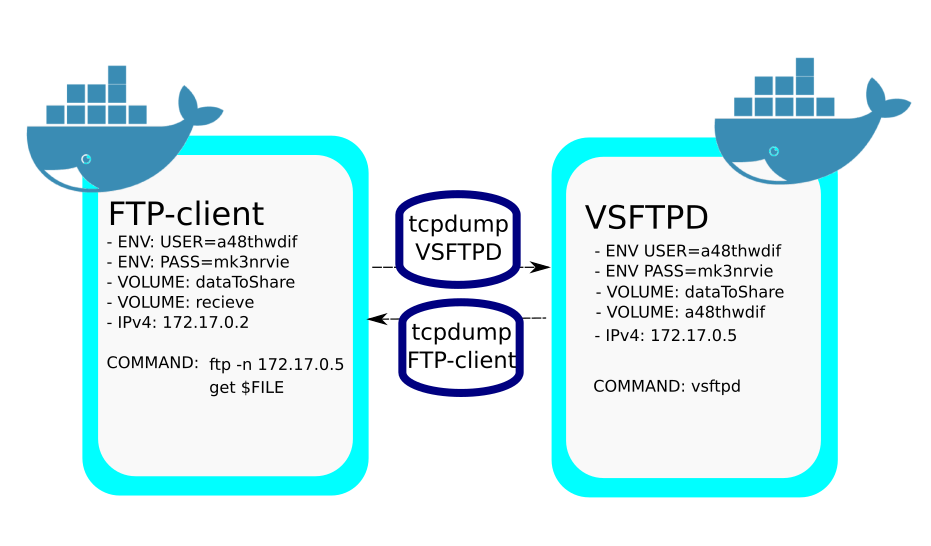
\includegraphics[width=0.50\textwidth]{images/ftp_example.png}
\caption{Diagram of our FTP scenario}
\end{figure}

We shall review the design of a prototypical capture scenario, namely, an FTP server and client interaction. The entire interaction is initiated by a single script, which allows the user to specify the length of the interaction, the number of times the interaction takes place as well as the specific scenario that should govern the interaction at runtime. Upon specifying these parameters, the script then generates a random ftp username and password, creating the necessary \textit{User} directory on the host machine before calling the docker-compose file which creates a user-defined bridge network. Subsequently, the necessary containers are then started which, in this case, consist of a vsftpd server, a client with ftp installed and two containers running tcpdump to capture all of the traffic emitted and received by the client and server respectively into separate .pcap files. These .pcap files are then sent to the host machine via a shared data directory. In addition, the host machine also shares:
    
\begin{itemize}
\item A \textit{dataToShare} volume containing files that can be downloaded by the client.
\item The \textit{User} directory with the server --- which contains the same files as the \textit{dataToShare} folder.
\item An empty \textit{recieve} folder with the client into which the files will be downloaded.
\item The random username and password is also shared with the client container to allow it to authenticate itself with the server.
\end{itemize}
    
    Up to this point, no network traffic has been generated and the containers are now ready to begin communicating with one another. 
    For this particular interaction between an FTP server and client, we want to ensure that it is possible to capture the many ways in which an FTP session may develop. For instance, the client may seek to download files via the \texttt{get} command or the \texttt{put} command, alongside many other possibilities. There are 13 possible capture scenarios intended to encapsulate a wide range of potential FTP sessions. These include downloading a single file using \texttt{get} or \texttt{put}, downloading every file using \texttt{mget} or \texttt{mput}, deleting every file from the server and requesting files from the server without the necessary authentication.

    Finally, after the scenario ends, both the \textit{User} directory and any downloaded files are then removed from the host machine. Following this, the containers are then stopped and the bridge network is torn down. All necessary containers, volumes and scripts are in the same position prior to initiating the scenario --- barring any generated .pcap files --- allowing for the scenarios to be started repeatedly with minimal human interaction.
        

\subsection{Dataset creation}
Write how to combine individual .pcap files to one dataset. Do we have a script for this?

\subsection{Existing scenarios}


\section{Validation experiments}

\subsection{Verification experiments - Henry}

Use Rob's Deterministic Scenarios section

\subsection{Exploration of Artificial Delays}

\subsection{Classifying Application Flows using IATs}
The name needs to be changed, be clear what this verifies about our framework


\section{Difficulties and limitations}

\section{Conclusion}


\subsection{Future work}

\subsection{Related work}

\section{Acknowledgments}

We are grateful for our ongoing collaboration with our industry partners (blinded) on this topic area, who provided both ongoing support and guidance to this work. Discussions with them have helped reinforce the need for a better evaluation and understanding of the possibilities that new intelligent tools can provide.

Full funding sources after currently blinded.

\bibliographystyle{ACM-Reference-Format}
  
\bibliography{ACSAC_DYNAMICS}

\appendix

\section{Result tables}





 

\end{document}
